\documentclass[11pt,a4paper]{article}
\usepackage[margin=2.2cm]{geometry}
\usepackage{amsmath}
\usepackage{graphicx}
\usepackage{booktabs}
\usepackage{float}
\usepackage[font=small,labelfont=bf]{caption}
\usepackage[hyphens]{url}
\usepackage[hidelinks]{hyperref}

% Figures are produced by figures/scripts/Figure_PMF_comparison.ipynb
\graphicspath{{../../plot/}}
\setlength{\emergencystretch}{2em}

\newcommand{\kJ}{\,kJ\,mol$^{-1}$}

\title{Leucine (SCL) membrane-partitioning PMFs:\\
estimator comparison, pooled counting, and concentration dependence}
\date{}

\begin{document}
\maketitle

\section{Data and conventions}

\begin{itemize}
  \item \textbf{Unbiased MD.} SCL at 0.2\,M (\texttt{scl}, 26 molecules) and 0.1\,M
  (\texttt{scl-1}, 13 molecules). Three trajectories, each split into three 200\,ns blocks
  (400--600, 600--800, 800--1000\,ns): nine blocks per concentration. Each block contains
  520\,000 (0.2\,M) or 260\,000 (0.1\,M) molecule-frames. Histograms use 1\,\AA{} bins of $|z|$
  ($+z$ and $-z$ folded by adding counts).
  \item \textbf{MD water reference.} 40--50\,\AA{} from the bilayer centre.
  \item \textbf{Umbrella sampling (US).} Leucine, two 50\,ns blocks, 38 windows per leaflet,
  WHAM with 0.25\,\AA{} bins. Each folded block is shifted so that its mean PMF over
  $|z|\ge 30$\,\AA{} is zero; blocks are then averaged and the SE is a block bootstrap.
  \item \textbf{Temperature.} $T = 303.15$\,K, so $k_BT = 2.52$\kJ.
  \item \textbf{Membrane reference.} Where used, every curve is shifted so that its own minimum
  within $|z| = 0$--20\,\AA{} is zero.
\end{itemize}

\section{Main findings}

\begin{enumerate}
  \item \textbf{Inside the membrane, all estimators agree.} With the membrane reference, every
  MD estimator reproduces the US shape over 0--20\,\AA{} (RMSD 0.56--0.58\kJ{} at 0.2\,M and
  0.35--0.37\kJ{} at 0.1\,M; Table~\ref{tab:us}). The estimators differ only in how they
  connect the membrane to water.
  \item \textbf{The water reference is the bottleneck.} Leucine rarely leaves the bilayer. At
  0.2\,M only 4/9 blocks visit the 40--50\,\AA{} window; at 0.1\,M only 1/9 blocks does
  (Table~\ref{tab:water}). Estimators that take the logarithm of each block separately must
  invent a value for the empty blocks (pseudocount, prior, or latent model). The resulting
  water reference, and hence the well depth, is controlled by that model.
  \item \textbf{At 0.2\,M, pooled counts superimpose best on US.} Pooled counts give a well depth
  of $-18.46 \pm 2.04$\kJ{} versus $-17.86 \pm 0.25$\kJ{} for US, and an RMSD of 0.56\kJ{} over
  0--38\,\AA{}. The other estimators give 2.4--6.7\kJ. Pooled counts are also the only MD
  estimator that reproduces the interfacial barrier: $+3.60$\kJ{} at 22.5\,\AA{}, versus
  $+3.52$\kJ{} at 22.1\,\AA{} for US. The other estimators give $\le 0.9$\kJ, shifted to 23.5--26.5\,\AA.
  \item \textbf{At 0.1\,M, no estimator reproduces US.} All MD curves are 5--16\kJ{} deeper
  than US. Pooled counts ($-23.28 \pm 1.14$\kJ, RMSD 4.13\kJ) no longer outperform the
  pseudocount (RMSD 3.98\kJ). The entire 0.1\,M membrane-to-water connection comes from
  one block containing 298 water-window counts.
  \item \textbf{The concentration difference is weakly supported.} With pooled counts, the
  0.2\,M and 0.1\,M curves agree within the membrane under the membrane reference: mean
  difference $+0.07 \pm 0.11$\kJ{} over 0--20\,\AA. Their membrane-to-water offset differs
  by about 3--5\kJ{} ($p \approx 0.02$--$0.05$; Section~\ref{sec:pvalues}). This evidence is
  conditional on the single water-visiting 0.1\,M block. Valine and isoleucine show no
  consistent concentration effect either (Section~\ref{sec:val_ile}).
\end{enumerate}

\begin{table}[H]
\centering
\caption{Molecule-frame counts in the 40--50\,\AA{} water window for each block
(T = trajectory, B = 200\,ns block).}
\label{tab:water}
\begin{tabular}{lccccccccc}
\toprule
 & T1/B1 & T1/B2 & T1/B3 & T2/B1 & T2/B2 & T2/B3 & T3/B1 & T3/B2 & T3/B3 \\
\midrule
0.2\,M & 0 & 1584 & 0 & 0 & 0 & 0 & 796 & 62 & 1818 \\
0.1\,M & 298 & 0 & 0 & 0 & 0 & 0 & 0 & 0 & 0 \\
\bottomrule
\end{tabular}
\end{table}

\section{Comparison of estimators with umbrella sampling}

Five MD estimators are compared:
\begin{itemize}
  \item a pseudocount, $-k_BT\ln(p+\varepsilon)$ with $\varepsilon = 10^{-5}$;
  \item Poisson--Gamma;
  \item Bayesian (Dirichlet);
  \item latent logarithm;
  \item pooled counts.
\end{itemize}
The first four average the logarithms of the nine block histograms. Pooled counts sum the
counts first and take a single logarithm.

\begin{figure}[H]
\centering
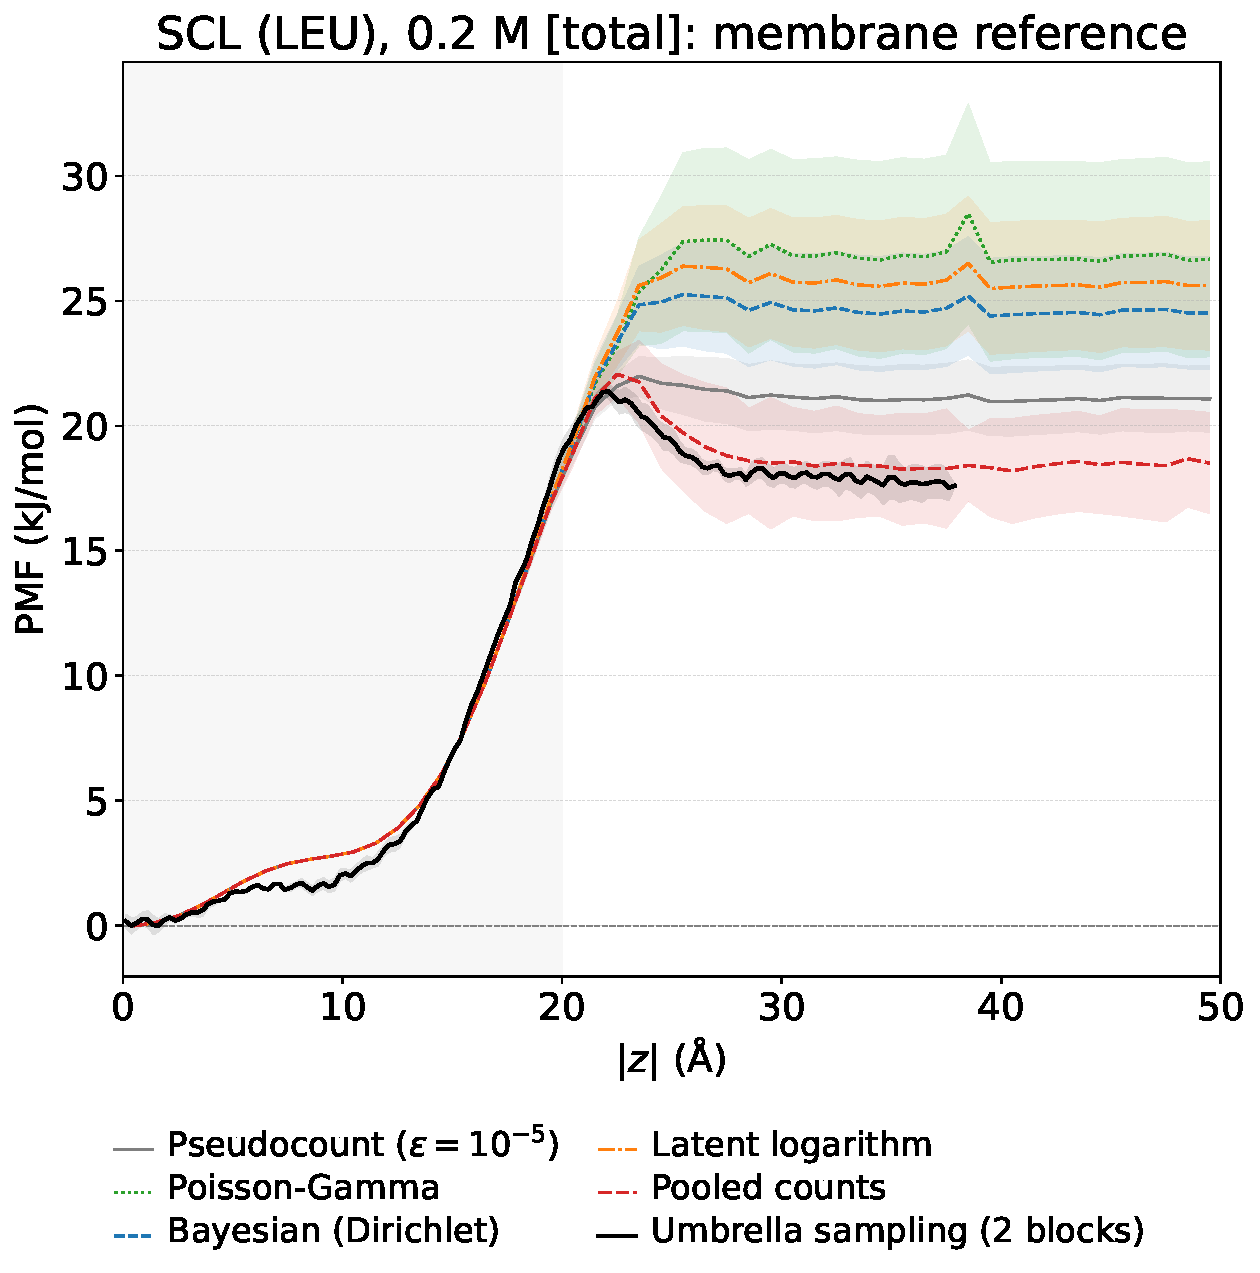
\includegraphics[width=0.49\textwidth]{FigureS_PMF_scl_methods_US_total_membrane}
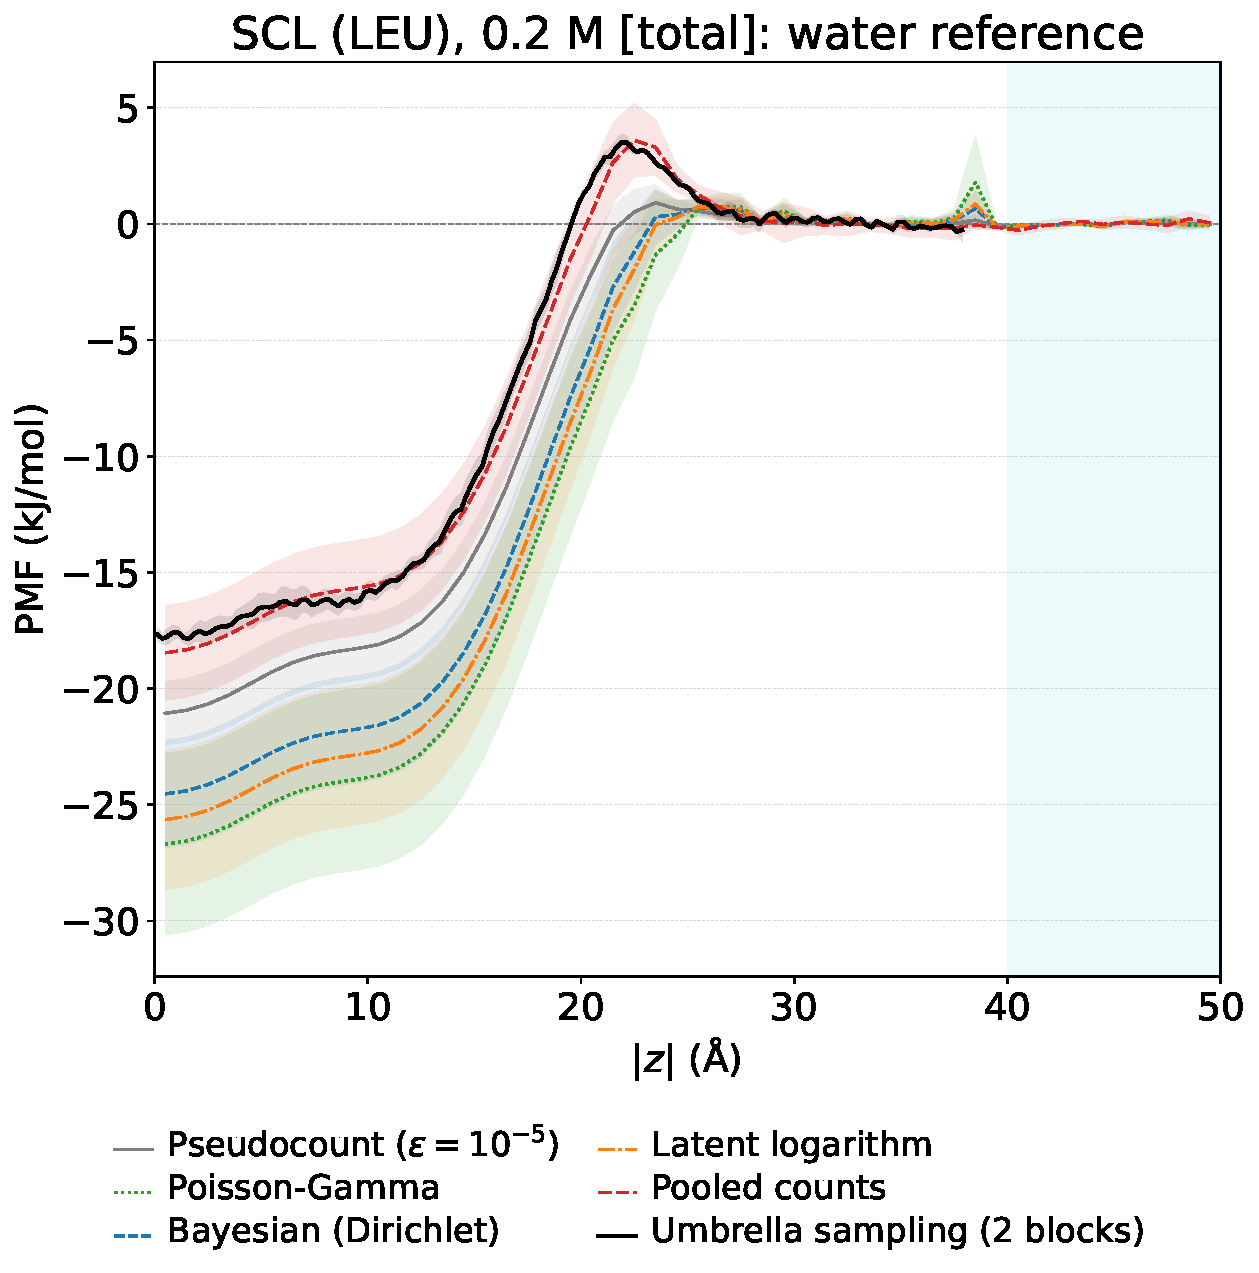
\includegraphics[width=0.49\textwidth]{FigureS_PMF_scl_methods_US_total_water}
\caption{SCL at 0.2\,M versus leucine US. Left: membrane reference (each minimum in
0--20\,\AA{} set to zero). All estimators coincide in the membrane, but their water plateaus
span 18--27\kJ; pooled counts (18.4\kJ) match the US plateau (17.9\kJ). Bands: untranslated
SE under a fixed shift; the uncertainty of each curve's minimum is not propagated. Right:
water reference (MD: 40--50\,\AA; US: each folded block set to zero over $|z|\ge30$\,\AA).
Pooled counts superimpose on US over the whole profile, including the barrier at 22\,\AA.
Bands: SE; the pooled-count SE excludes bootstrap replicates without water counts.}
\label{fig:methods02}
\end{figure}

\begin{table}[H]
\centering
\caption{Agreement with US (kJ\,mol$^{-1}$). The US curve is averaged into the 1\,\AA{} MD bins
over 0--38\,\AA{}. ``Min'' is the water-referenced minimum $\pm$ SE (US: $-17.86 \pm 0.25$).
``RMSD$_w$'' and ``RMSD$_m$'' use the water and membrane references, over 0--38\,\AA{} and
0--20\,\AA, respectively. ``Barrier'' is the maximum over 18--30\,\AA{} (US: $+3.52$).}
\label{tab:us}
\small
\setlength{\tabcolsep}{4pt}
\begin{tabular}{l rrrr rrr}
\toprule
 & \multicolumn{4}{c}{0.2\,M} & \multicolumn{3}{c}{0.1\,M} \\
\cmidrule(lr){2-5}\cmidrule(lr){6-8}
Estimator & Min & RMSD$_w$ & RMSD$_m$ & Barrier & Min & RMSD$_w$ & RMSD$_m$ \\
\midrule
Pseudocount   & $-21.07 \pm 1.37$ & 2.44 & 0.57 & 0.92 & $-23.19 \pm 0.71$ & 3.98 & 0.35 \\
Poisson--Gamma& $-26.70 \pm 3.91$ & 6.72 & 0.56 & 0.74 & $-33.63 \pm 2.22$ & 12.04 & 0.36 \\
Bayesian      & $-24.54 \pm 2.31$ & 5.01 & 0.56 & 0.72 & $-26.90 \pm 1.16$ & 6.69 & 0.36 \\
Latent        & $-25.64 \pm 3.01$ & 5.85 & 0.56 & 0.75 & $-29.57 \pm 1.80$ & 8.67 & 0.37 \\
Pooled counts & $\mathbf{-18.46 \pm 2.04}$ & \textbf{0.56} & 0.58 & \textbf{3.60} & $-23.28 \pm 1.14$ & 4.13 & 0.36 \\
\bottomrule
\end{tabular}
\end{table}

\paragraph{Why do the log-averaging estimators give deeper wells?}
They estimate the water probability block by block. A block that never reaches water would
give $\ln 0$. Each method therefore assigns that block a small value instead: the
pseudocount, the prior, or the latent model. These values are much smaller than the
probability observed in water-visiting blocks. Averaging the logarithms then makes the
water reference less favourable, and the well appears deeper. The magnitude depends on the
zero-handling model, not on additional observations. Pooled counts treat a block without
water visits as observation time with zero visits; they do not need a value for $\ln 0$.

\section{The pooled-count method}

\subsection{Principle}
Let $n_b(z)$ be the number of molecule-frames observed in bin $z$ during block $b$. The
pooled-count PMF is
\begin{align}
C(z) &= \sum_{b=1}^{9} n_b(z) && \text{(sum counts \emph{before} the logarithm)}\\
P(z) &= \frac{C(z)}{\sum_{z'} C(z')} && \text{(normalise over the full native grid)}\\
a &= -k_BT \ln \big\langle P \big\rangle_{40\text{--}50\,\text{\AA}} && \text{(water reference)}\\
G(z) &= -k_BT\ln P(z) - a = -k_BT\ln\frac{C(z)}{\langle C\rangle_{40\text{--}50\,\text{\AA}}}.
\end{align}
\begin{itemize}
  \item No pseudocount is added.
  \item No block is discarded. Blocks with zero counts in a bin contribute observation time.
  \item A bin with no counts in any block remains undefined.
  \item No PMF curves are averaged.
  \item Because all blocks have the same depth, pooling is equivalent to averaging the block
  \emph{probabilities} before the logarithm. It is not equivalent to averaging the block
  PMFs: $-k_BT\ln\bar p \ne \overline{-k_BT\ln p}$.
\end{itemize}

\subsection{Step-by-step construction for SCL at 0.2\,M}

\begin{figure}[!htbp]
\centering
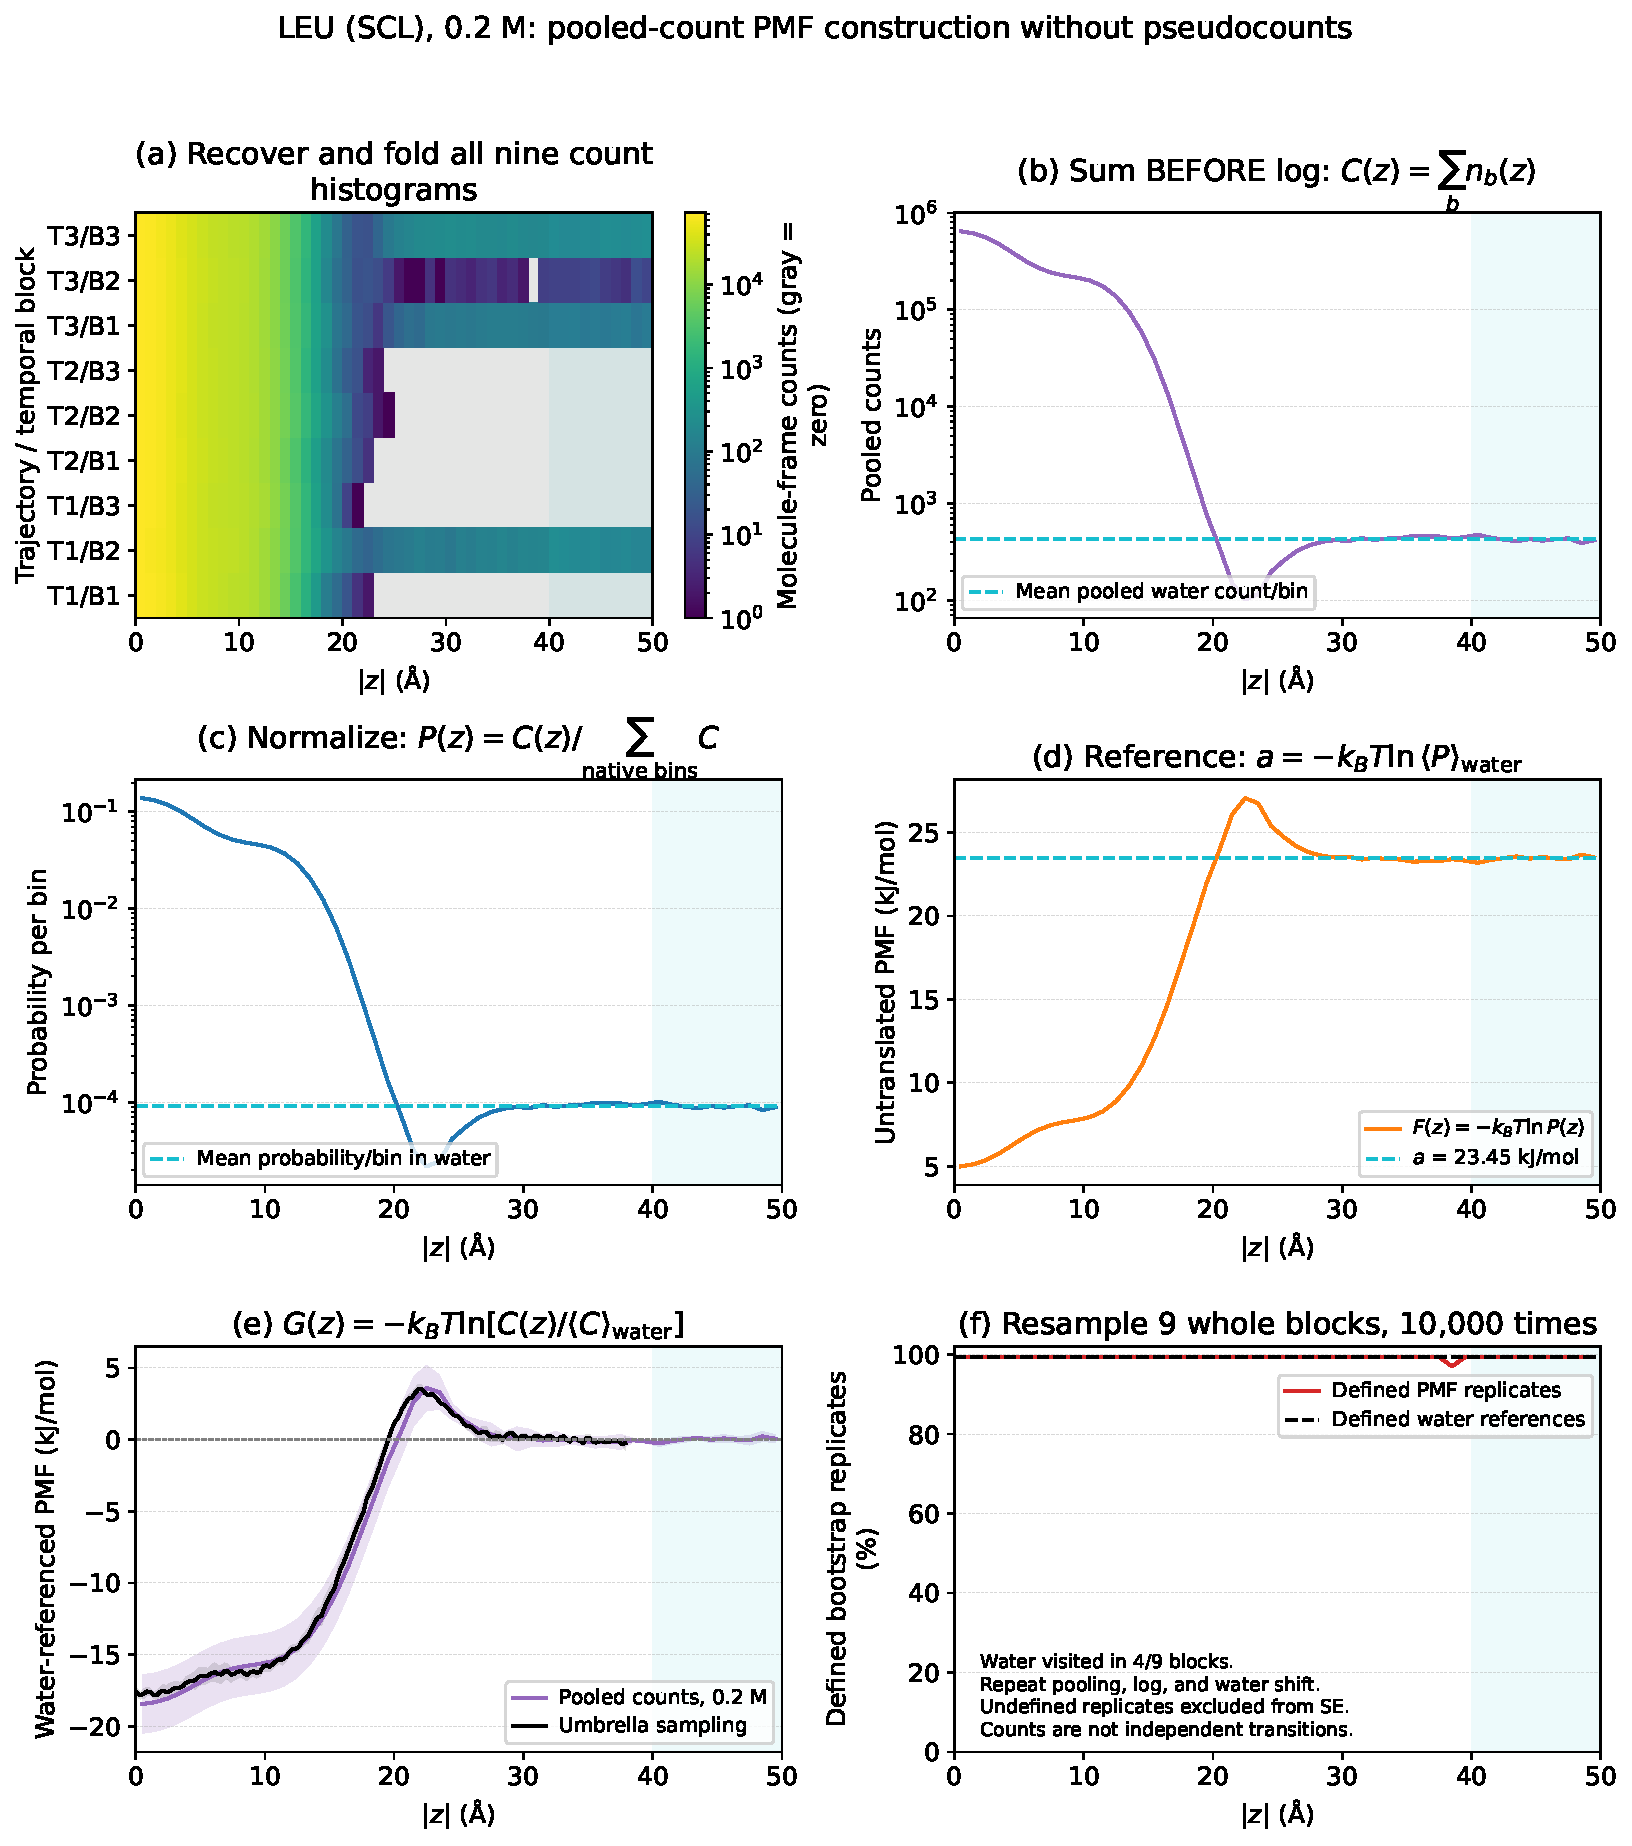
\includegraphics[width=\textwidth]{FigureS_PMF_pooled_counts_steps_scl_total}
\caption{Pooled-count construction for SCL at 0.2\,M. All nine blocks are retained; grey
cells in (a) are observed non-visits, not missing records. The water reference uses the mean
probability per bin, not the mean PMF. SE: block bootstrap (defined replicates only)
$\times\sqrt{9/8}$; temporal correlation and unvisited states remain limitations.}
\label{fig:steps02}
\end{figure}

Figure~\ref{fig:steps02} shows the procedure:
\begin{enumerate}
  \renewcommand{\labelenumi}{(\alph{enumi})}
  \item \textbf{Recover and fold all nine count histograms.} Each normalised histogram is
  multiplied by the block depth to recover integer counts; rounding and total counts are
  checked. Grey cells are \emph{observed non-visits}, not missing data.   Five blocks never go beyond 25\,\AA.
  \item \textbf{Sum before the logarithm.} The total is 4\,680\,000 molecule-frames. Water bins
  contain about 426 pooled counts each, compared with about $6\times 10^5$ at the
  bilayer centre.
  \item \textbf{Normalise.} The mean water probability per bin is about $9\times10^{-5}$.
  \item \textbf{Water reference.} $F(z) = -k_BT\ln P(z)$ and $a = -k_BT\ln\langle P\rangle_\text{water}
  = 23.45 \pm 2.04$\kJ. The reference uses the mean \emph{probability} per bin, not the mean
  PMF, so individual water bins fluctuate around zero.
  \item \textbf{Water-referenced PMF.} $G = F - a$ superimposes on US, including the
  barrier at about 22\,\AA.
  \item \textbf{Uncertainty.} The nine blocks are resampled with replacement 10\,000 times, and
  pooling, logarithm, and reference are repeated each time. A replicate is undefined when it
  contains no water-visiting block. Here, the probability of drawing none of the four
  water-visiting blocks is $(5/9)^9 = 0.5\%$; the observed defined fraction is 99.39\%.
  The SE uses defined replicates only and is multiplied by $\sqrt{n/(n-1)}=\sqrt{9/8}$.
\end{enumerate}

\section{SCL at 0.1\,M}

\begin{figure}[H]
\centering
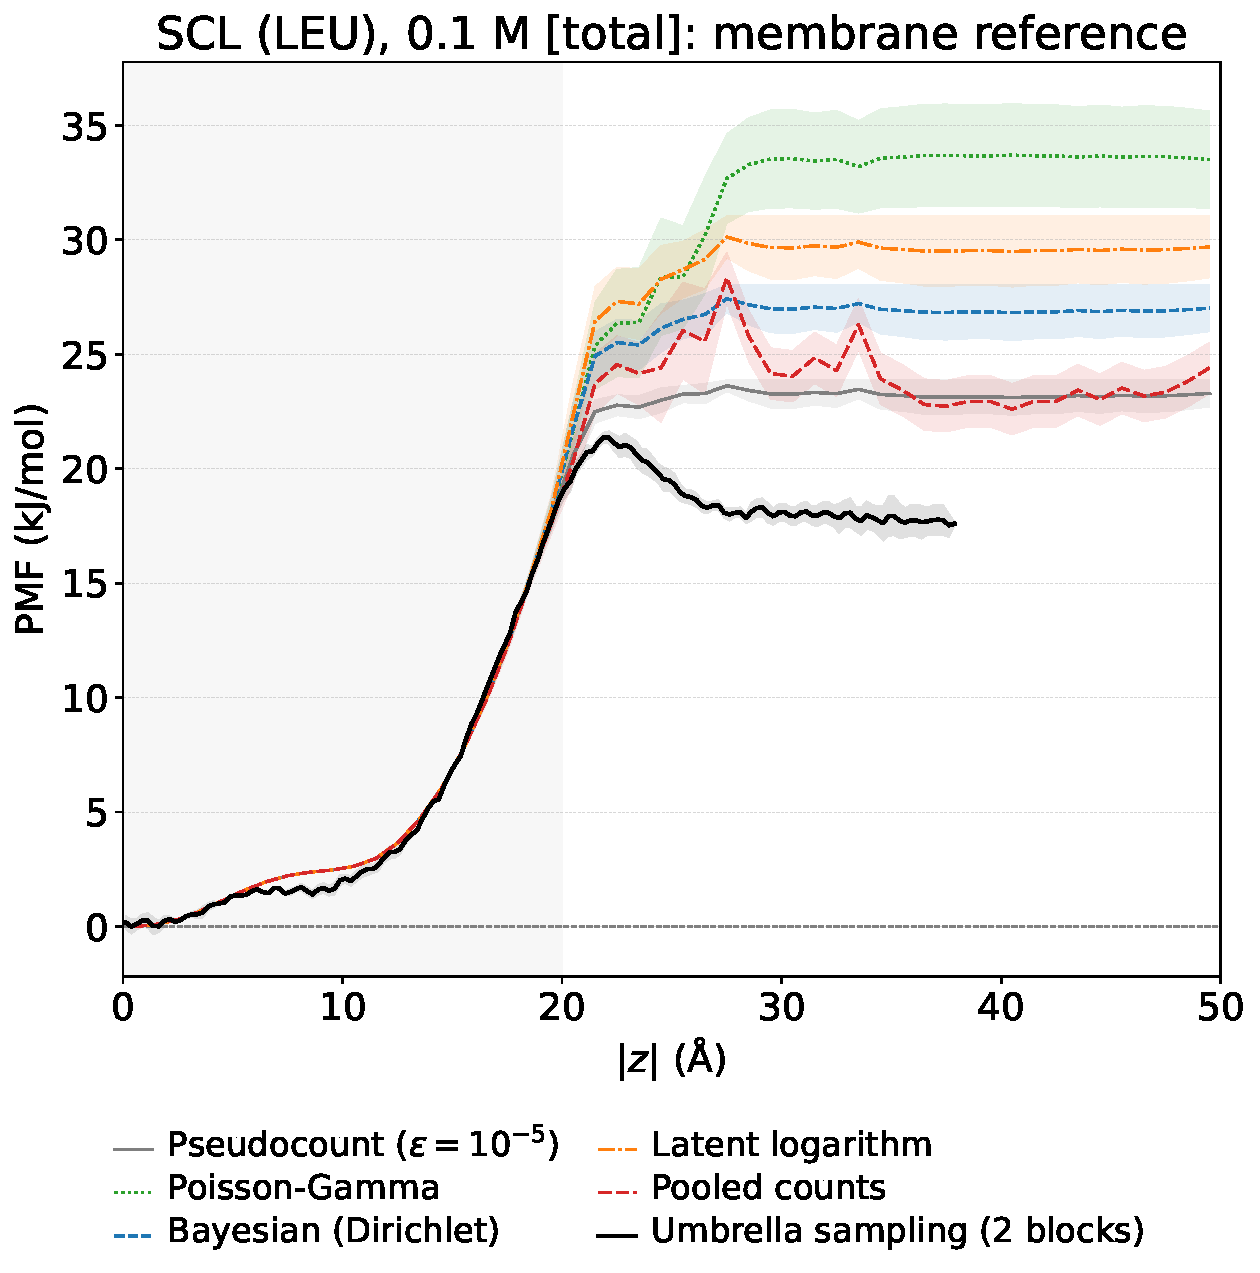
\includegraphics[width=0.49\textwidth]{FigureS_PMF_scl_01M_methods_US_total_membrane}
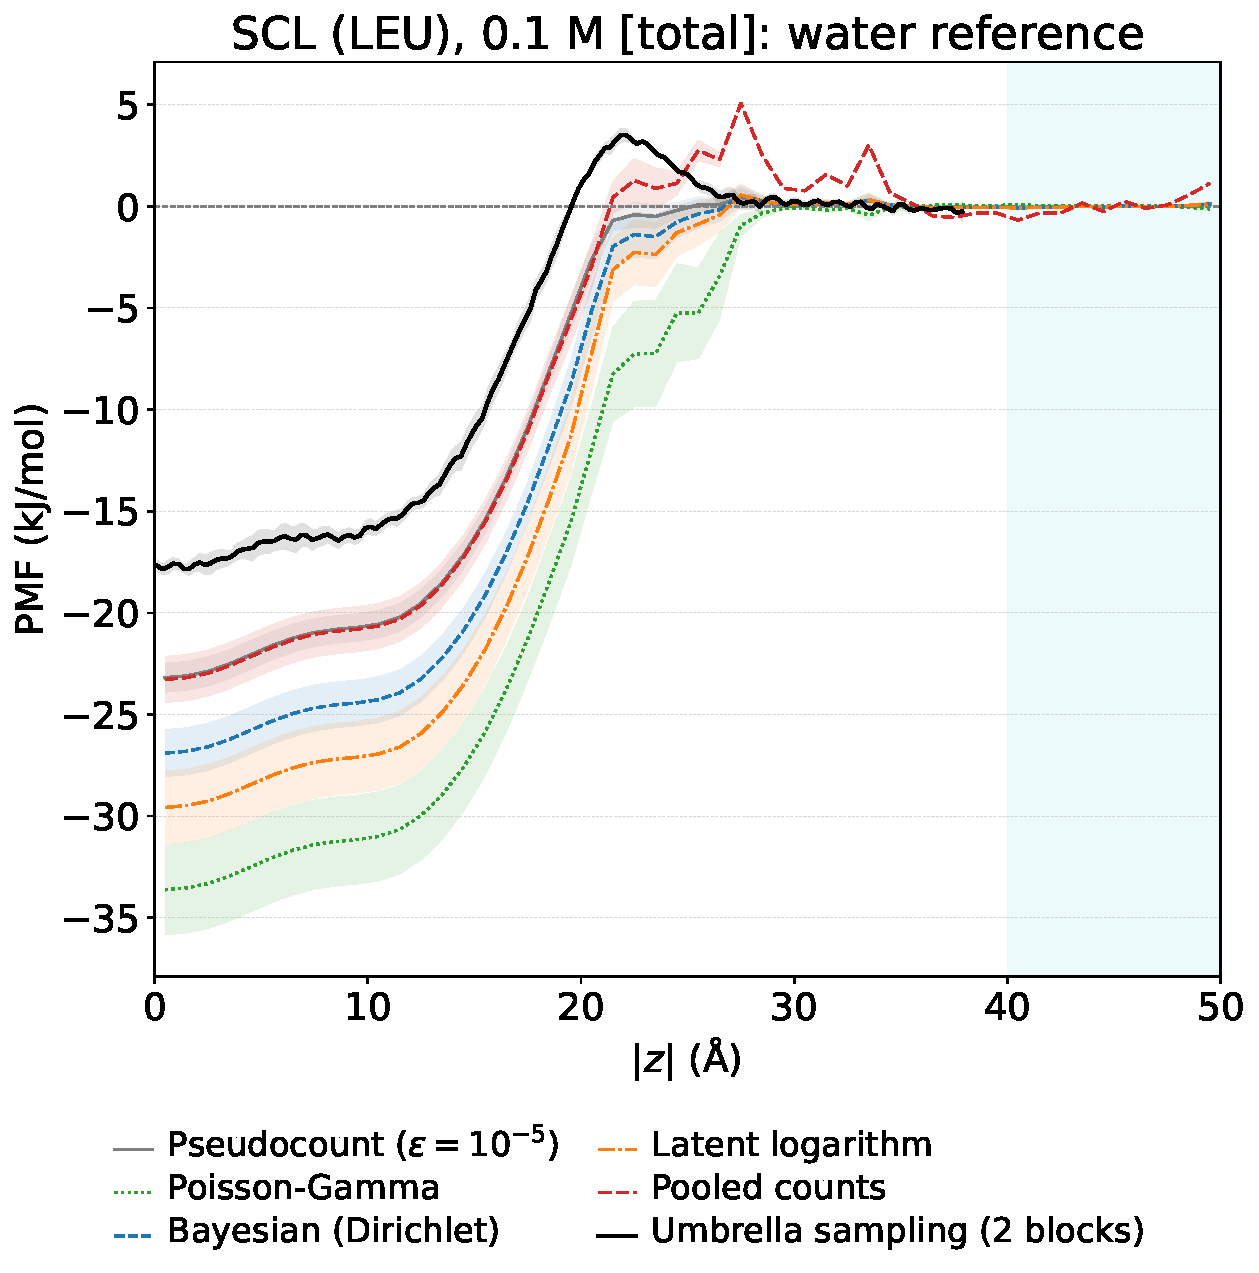
\includegraphics[width=0.49\textwidth]{FigureS_PMF_scl_01M_methods_US_total_water}
\caption{SCL at 0.1\,M versus leucine US. Left: membrane reference; all estimators coincide
up to 20\,\AA, then reach water plateaus of 23--34\kJ{} (US: 17.9\kJ). Bands: untranslated SE
under a fixed shift; the uncertainty of each curve's minimum is not propagated. Right: water
reference (MD: 40--50\,\AA; US: each folded block set to zero over $|z|\ge30$\,\AA); every MD
estimator is deeper than US. Pooled counts show spikes at 27--34\,\AA{} where only a few
counts exist. Bands: SE; the pooled-count SE excludes bootstrap replicates without water
counts (only 65.4\% of replicates are defined).}
\label{fig:methods01}
\end{figure}

\begin{figure}[!htbp]
\centering
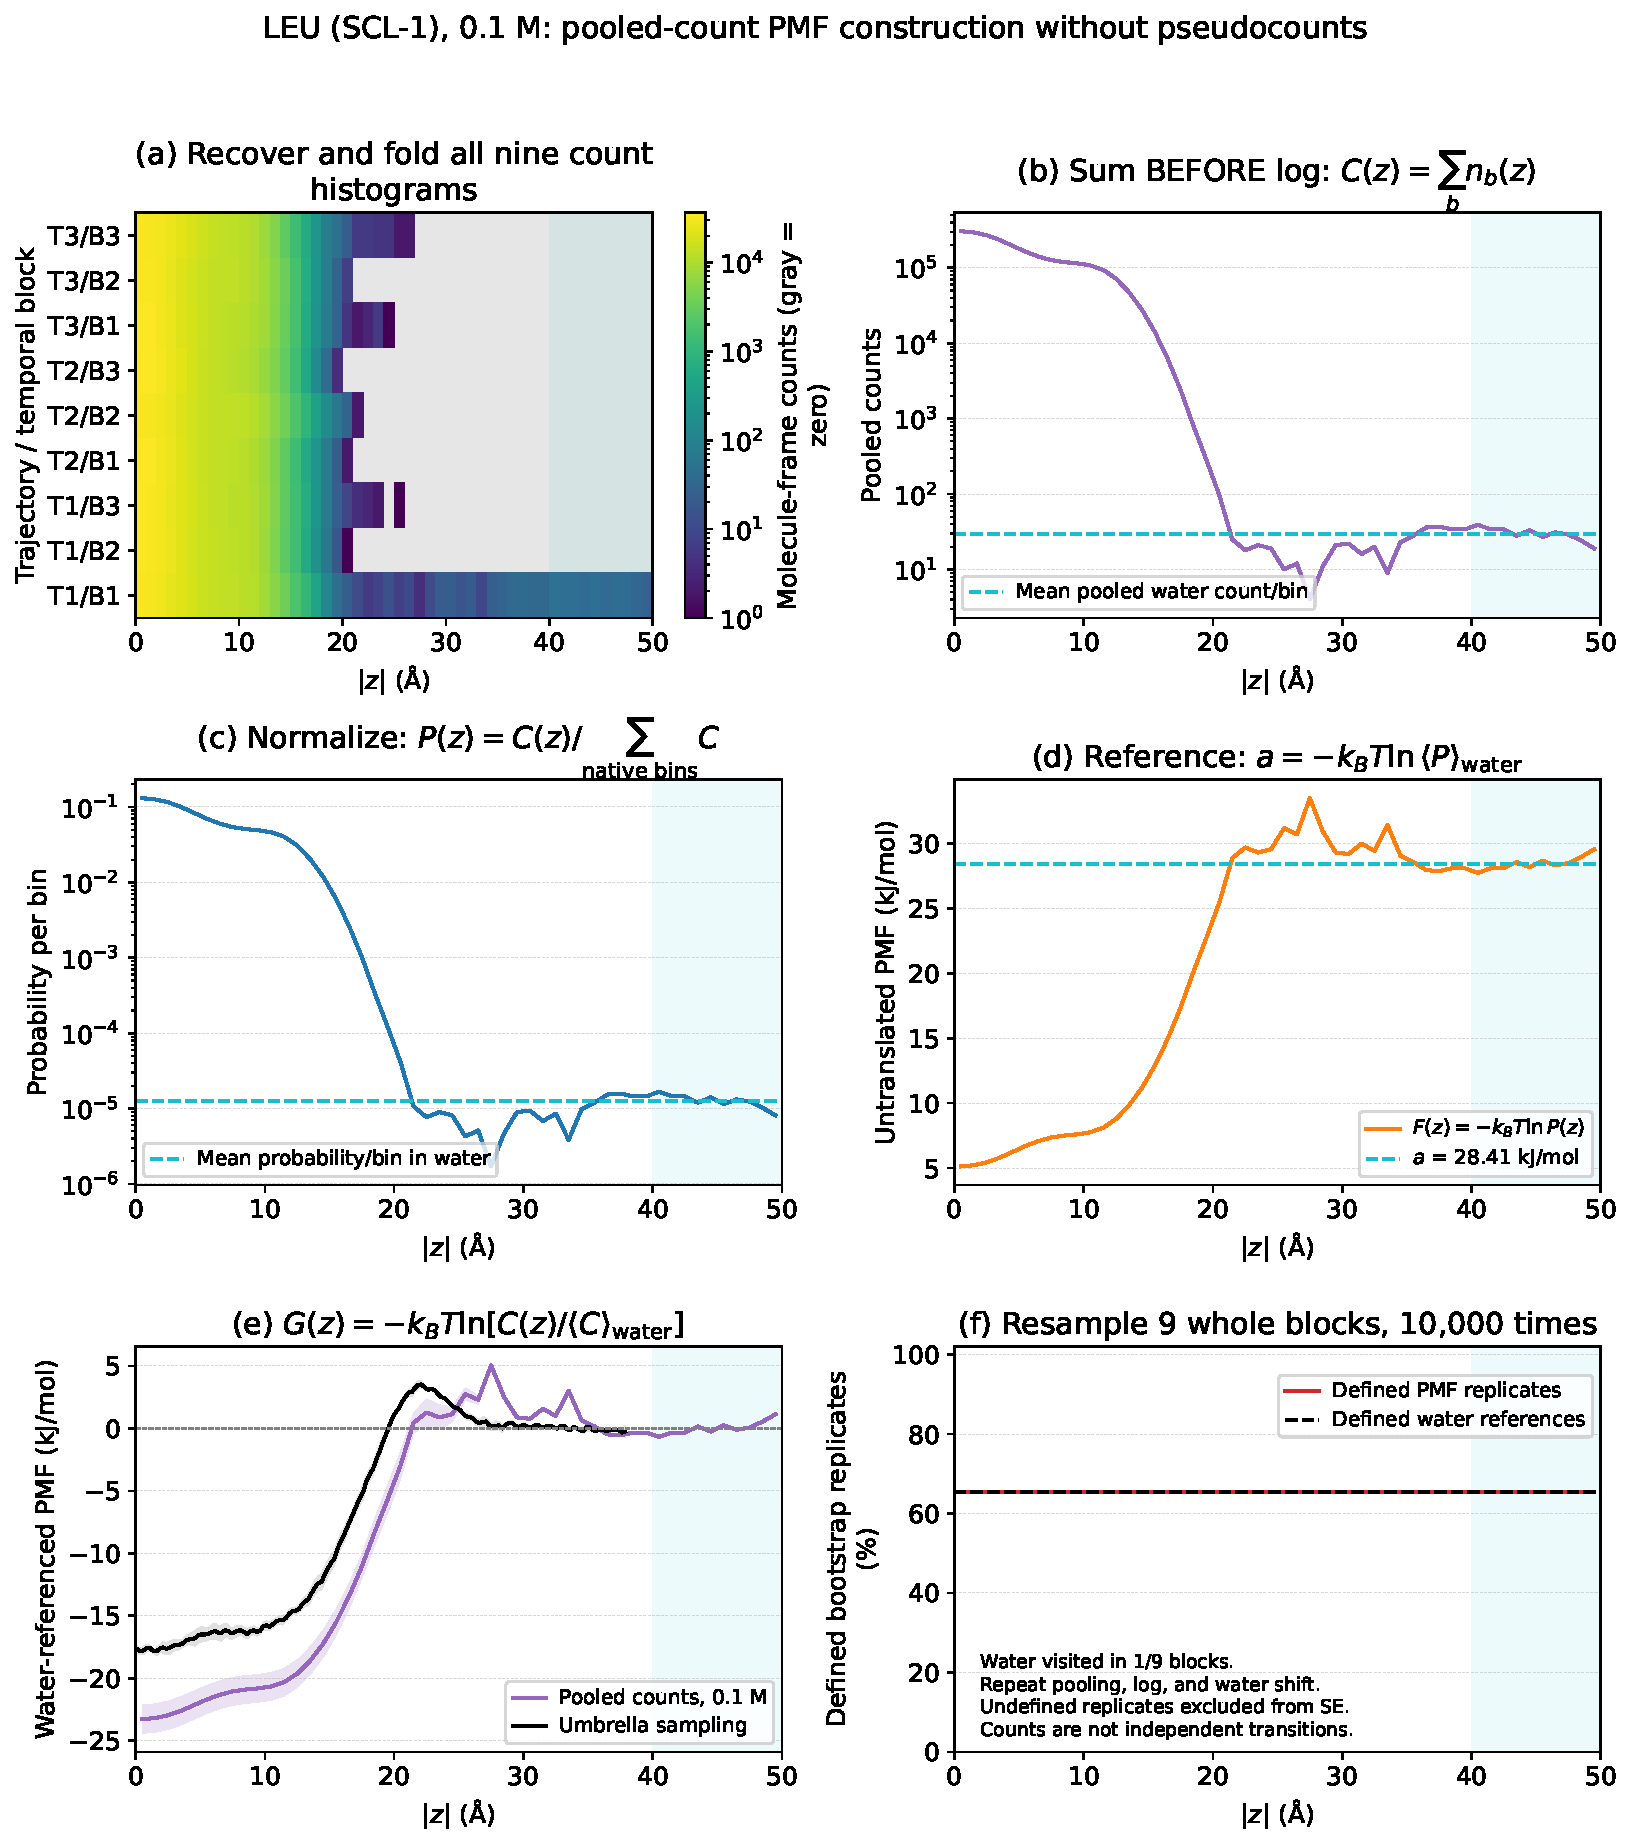
\includegraphics[width=\textwidth]{FigureS_PMF_pooled_counts_steps_scl-1_total}
\caption{Pooled-count construction for SCL at 0.1\,M. Conventions as in
Figure~\ref{fig:steps02}: all nine blocks retained, grey cells are observed non-visits, the
water reference is the mean probability per bin, and the SE uses defined bootstrap
replicates only $\times\sqrt{9/8}$.}
\label{fig:steps01}
\end{figure}

Figure~\ref{fig:steps01} shows why 0.1\,M is harder:
\begin{itemize}
  \item \textbf{Panel (a).} Only T1/B1 goes beyond about 27\,\AA; every water count comes from
  that single block.
  \item \textbf{Panels (b)--(d).} Pooled water counts are about 30 per bin, and
  $a = 28.41 \pm 1.12$\kJ.
  \item \textbf{Panel (f).} A bootstrap replicate is defined only when it contains T1/B1. The
  probability of missing it is $(8/9)^9 = 34.6\%$; the observed defined fraction is 65.4\%.
  The SE is therefore conditional on drawing that block. Its spread reflects only how many
  copies of T1/B1 are drawn, not the uncertainty about whether other trajectories would
  visit water. It probably underestimates the true uncertainty of the well depth.
\end{itemize}

\begin{figure}[!htbp]
\centering
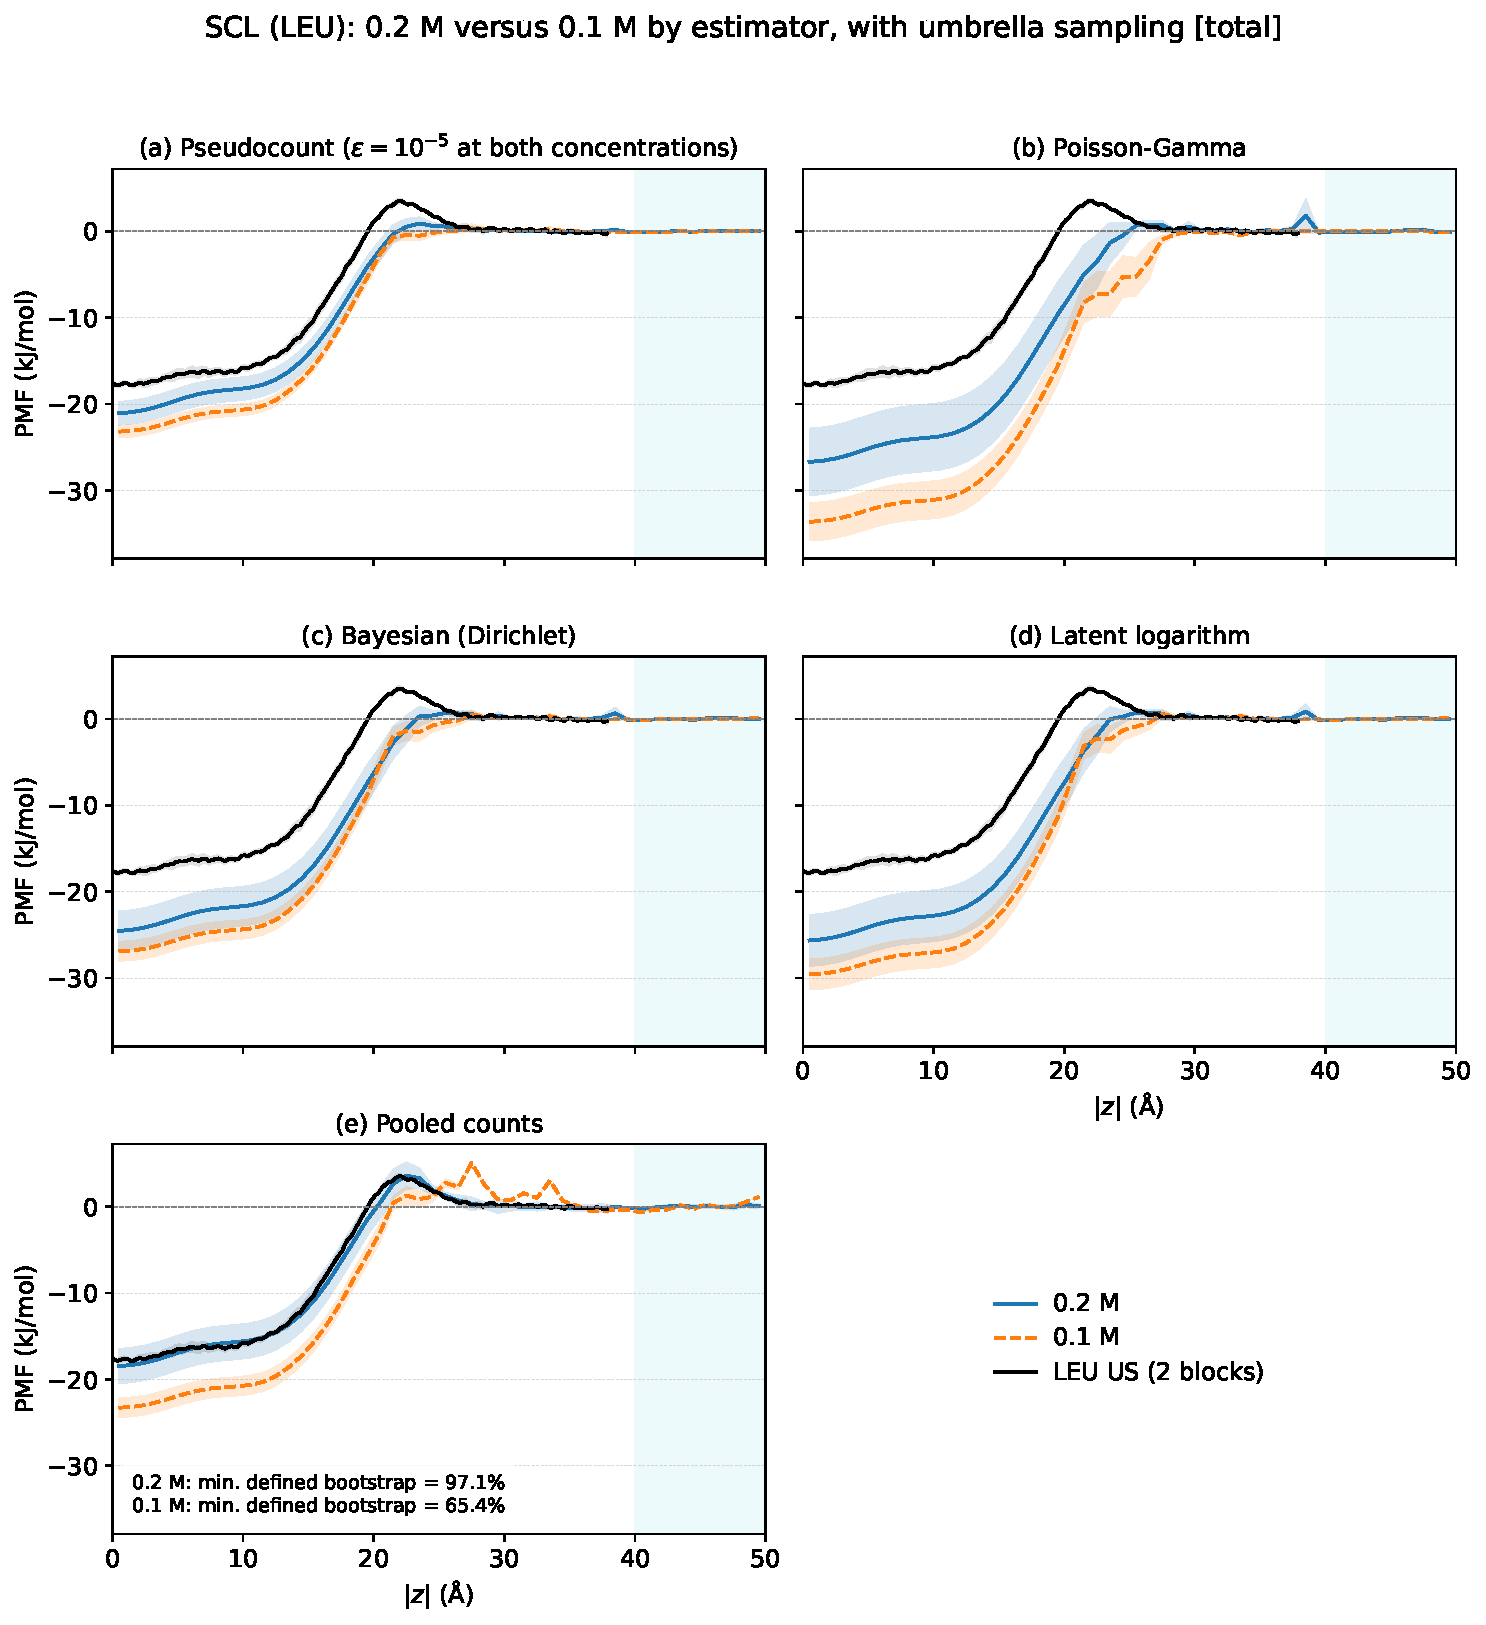
\includegraphics[width=\textwidth]{FigureS_PMF_scl_concentration_methods_US_total}
\caption{SCL at 0.2\,M versus 0.1\,M for each estimator, water reference, with leucine US.
For every estimator, 0.1\,M is deeper than 0.2\,M. Only the pooled-count 0.2\,M curve
coincides with US. Water references: MD 40--50\,\AA; US each folded block set to zero over
$|z|\ge30$\,\AA. Bands: SE; the pooled-count SE excludes bootstrap replicates without water
counts.}
\label{fig:conc}
\end{figure}

\section{Is the concentration effect significant?}
\label{sec:pvalues}

\subsection{Test}
The test uses pooled counts. For each concentration, the nine blocks are resampled
independently 10\,000 times. In each replicate, the pooled PMF and its reference are recomputed.
For the membrane reference, the reference is the minimum within 0--20\,\AA; for the water
reference, it is the mean 40--50\,\AA{} probability. The difference
$\Delta G(z) = G_{0.2\,\text{M}}(z) - G_{0.1\,\text{M}}(z)$ is tested over two regions,
0--20\,\AA{} and 0--50\,\AA, using two bootstrap statistics:
\begin{itemize}
  \item \textbf{$p(\max|t|)$:} the largest studentised local difference, sensitive to a
  difference in any single bin;
  \item \textbf{$p(\text{offset})$:} the region-averaged difference, sensitive to a systematic
  vertical shift.
\end{itemize}
Both use the centred bootstrap null distribution. Replicates with an undefined bin in the
region are excluded.

The two references contain the same membrane-to-water free-energy difference. Changing the
reference only moves where that difference appears: in water for the membrane reference, or
in the membrane for the water reference. Different p-values therefore reflect the region
being compared, not a different physical result.

\begin{figure}[H]
\centering
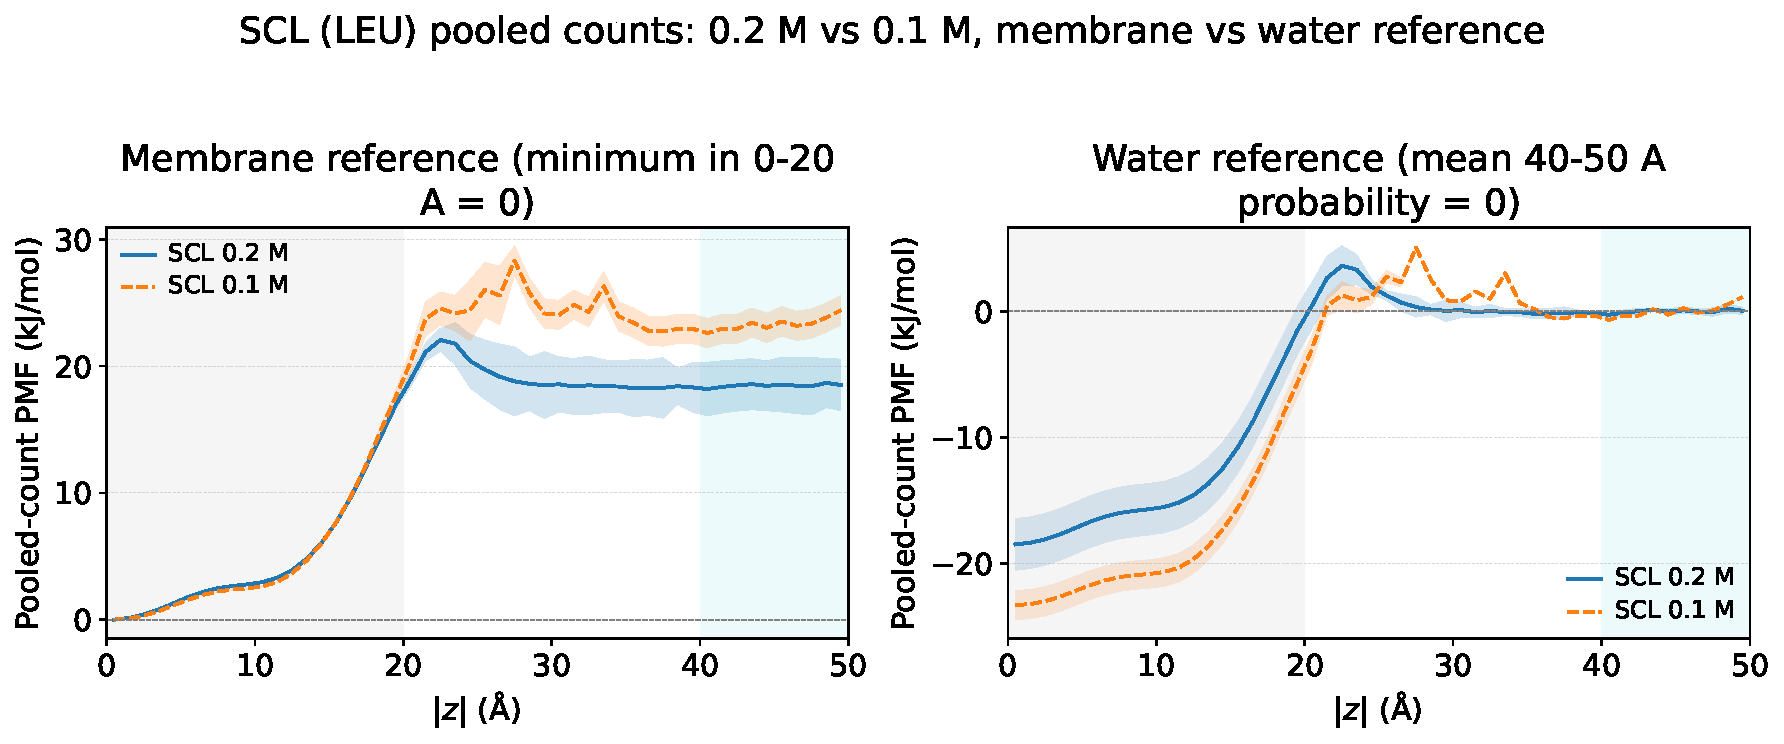
\includegraphics[width=\textwidth]{FigureS_PMF_scl_concentration_pvalues_total}
\caption{Pooled-count PMFs of SCL at 0.2 and 0.1\,M with the membrane reference (left) and
the water reference (right). Grey: 0--20\,\AA; cyan: 40--50\,\AA{} water window. Bands:
block-bootstrap SE (defined replicates only) $\times\sqrt{9/8}$, with the reference
re-estimated in every replicate. The tests of $G_{0.2\,\text{M}} - G_{0.1\,\text{M}}$ are
given in Table~\ref{tab:pvalues}.}
\label{fig:pvalues}
\end{figure}

\begin{table}[H]
\centering
\caption{Bootstrap tests of $G_{0.2\,\text{M}} - G_{0.1\,\text{M}}$ for pooled counts
(kJ\,mol$^{-1}$). p-values: centred bootstrap, 10\,000 independent resamples per
concentration; replicates with undefined bins are excluded. The smallest attainable
$p(\max|t|)$ is $1/(1+n_\text{defined})$, i.e.\ $10^{-4}$ or $1.6\times10^{-4}$, so values at
that limit are reported as an upper bound.}
\label{tab:pvalues}
\begin{tabular}{llrrrrr}
\toprule
Reference & Region & Mean $\Delta G$ & Max $|\Delta G|$ & $p(\max|t|)$ & $p(\text{offset})$ & Defined \\
\midrule
Membrane & 0--20\,\AA & $+0.07 \pm 0.11$ & 0.66 & $\le 0.0001$ & 0.52 & 100.0\% \\
Membrane & 0--50\,\AA & $-2.99 \pm 1.02$ & 9.53 & $\le 0.0002$ & 0.024 & 63.8\% \\
Water    & 0--20\,\AA & $+4.89 \pm 2.29$ & 5.15 & 0.053 & 0.051 & 65.3\% \\
Water    & 0--50\,\AA & $+1.82 \pm 0.80$ & 5.15 & $\le 0.0002$ & 0.080 & 63.8\% \\
\bottomrule
\end{tabular}
\end{table}

\paragraph{Interpretation.}
\begin{itemize}
  \item \textbf{Membrane shape (membrane reference, 0--20\,\AA).} The curves have the same
  shape: mean difference $+0.07\pm0.11$\kJ, $p(\text{offset}) = 0.52$. The small
  $p(\max|t|)$ reflects local differences of at most 0.66\kJ{} ($0.26\,k_BT$). These are
  detectable only because the membrane is densely sampled, and they are physically
  negligible.
  \item \textbf{Membrane-to-water offset.} The water plateau of the membrane-referenced 0.1\,M
  curve lies about 3--5\kJ{} above that at 0.2\,M. Equivalently, the 0.1\,M water-referenced
  well is about 5\kJ{} deeper. This offset is borderline: $p = 0.024$ for the membrane
  reference over 0--50\,\AA{} and $p \approx 0.05$ for the water reference over 0--20\,\AA.
  \item \textbf{Local differences at 25--35\,\AA.} The small $p(\max|t|)$ values for both
  0--50\,\AA{} tests are driven by isolated interfacial spikes in the 0.1\,M curve, where
  a single block contributes only a few counts.
  \item \textbf{Conclusion.} The data do not establish a robust concentration effect on
  the leucine transfer free energy. The apparent effect relies on one 0.1\,M water-visiting
  block, and its p-values are conditional on drawing that block. More 0.1\,M sampling of the
  water phase, such as longer or additional trajectories, would be needed.
\end{itemize}

\section{Valine and isoleucine}
\label{sec:val_ile}

The same pooled-count analysis and bootstrap tests (Section~\ref{sec:pvalues}) were applied to
valine and isoleucine.
Table~\ref{tab:val_ile} compares them with leucine.

\begin{table}[H]
\centering
\caption{Pooled-count results at 0.2 and 0.1\,M (kJ\,mol$^{-1}$). ``Water blocks'': blocks
with counts in the 40--50\,\AA{} window (out of 9). ``Well'': water-referenced minimum
$\pm$ SE. $\Delta G = G_{0.2\,\text{M}} - G_{0.1\,\text{M}}$, mean over 0--20\,\AA{} $\pm$
bootstrap SE, with $p(\text{offset})$ in parentheses; a positive value means a deeper well at
0.1\,M. ``Shape'': membrane reference; ``offset'': water reference.}
\label{tab:val_ile}
\small
\setlength{\tabcolsep}{4pt}
\begin{tabular}{lccccc}
\toprule
Residue & Water blocks & Well, 0.2\,M & Well, 0.1\,M & $\Delta G$ shape & $\Delta G$ offset \\
\midrule
LEU & 4 / 1 & $-18.46 \pm 2.04$ & $-23.28 \pm 1.14$ & $+0.07 \pm 0.11$ (0.52) & $+4.89 \pm 2.29$ (0.051)$^{a}$ \\
VAL & 7 / 7 & $-17.54 \pm 1.13$ & $-13.95 \pm 1.13$ & $-0.01 \pm 0.07$ (0.93) & $-3.59 \pm 1.59$ (0.031) \\
ILE & 4 / 0 & $-19.46 \pm 1.95$ & undefined & $-0.11 \pm 0.08$ (0.16) & not testable \\
\bottomrule
\multicolumn{6}{l}{\footnotesize $^{a}$Conditional on the 65.3\% of replicates that contain the only
water-visiting 0.1\,M block.}
\end{tabular}
\end{table}

\paragraph{What has been demonstrated.}
\begin{itemize}
  \item \textbf{Inside the membrane, the PMF does not depend on concentration.} With the
  membrane reference, the 0--20\,\AA{} curves coincide for all three residues: mean
  differences are at most 0.11\kJ{} and none of the offsets is significant
  ($p = 0.16$--$0.93$). The only detectable local differences are $\le 1.2$\kJ{}
  ($\le 0.5\,k_BT$).
  \item \textbf{The membrane-to-water offset shows no consistent concentration effect.}
  Valine is the best-sampled case: 7/9 blocks reach water at both concentrations, and all
  bootstrap replicates are defined. Its 0.1\,M well is \emph{shallower} by
  $3.6 \pm 1.6$\kJ{} ($p = 0.031$), whereas the leucine 0.1\,M well is \emph{deeper} by
  $4.9 \pm 2.3$\kJ{} ($p = 0.051$). The two residues change in opposite directions.
  \item \textbf{The individual p-values are weak evidence.} Nine region/reference tests were
  run across the three residues, each with two statistics, without correction for multiple
  testing. Isolated values of $p \approx 0.03$ are therefore compatible with chance.
  \item \textbf{Isoleucine at 0.1\,M cannot be referenced to water.} None of its nine blocks
  reaches the 40--50\,\AA{} window, and no block has counts beyond 24.5\,\AA. The 0.1\,M
  transfer free energy is not estimable from these simulations, so only the membrane shape
  can be compared.
\end{itemize}

\paragraph{Conclusion.} Across leucine, valine, and isoleucine, halving the concentration
leaves the membrane profile unchanged. Apparent changes in the membrane-to-water free energy
are of similar size (3--5\kJ) but opposite sign, and they arise where water sampling is
sparsest. They are more consistent with limited water sampling than with a systematic
concentration effect. Resolving such an effect would require more water-phase sampling at
0.1\,M, especially for leucine and isoleucine.

\section{Which reference for hydrophobic residues?}
\label{sec:reference}

For the hydrophobic residues (leucine, valine, isoleucine), the \textbf{membrane reference}
should be used to compare PMF shapes between estimators, concentrations, and umbrella sampling.
It is anchored where the data are: the bilayer centre holds up to $6\times10^5$ pooled counts
per bin, whereas the water window holds about 430 per bin at 0.2\,M, 30 at 0.1\,M, and none for
isoleucine at 0.1\,M. With the water reference, this sparse water sampling shifts the whole
curve: the leucine 0--20\,\AA{} concentration difference is $+0.07 \pm 0.11$\kJ{} with the
membrane reference but $+4.89 \pm 2.29$\kJ{} with the water reference (Table~\ref{tab:pvalues}),
and the five estimators, which coincide inside the membrane, differ by up to 10.4\kJ{} because
each fills the empty water blocks differently. The membrane reference also remains defined when
water is never reached, and it loses no information: the membrane-to-water free energy appears
as the height of the water plateau, with its uncertainty confined to that region. The transfer
free energy itself, which requires the water reference, should be reported separately with the
pooled-count estimator, its bootstrap SE, and the number of blocks that reach water, and flagged
as unreliable when few blocks do (e.g.\ leucine at 0.1\,M, 1/9 blocks).

\section{Limitations}
\begin{itemize}
  \item Counts are molecule-frames, not independent events; a long excursion contributes many
  correlated counts. The autocorrelation function (ACF) shows that the trajectories decorrelate
  after about 50\,ns, so consecutive 200\,ns blocks within a trajectory can be treated as
  approximately independent. Rare membrane--water transitions may still be correlated over
  longer times.
  \item Bootstrap SEs and p-values exclude undefined replicates. They are conditional and do
  not represent the probability that a region is never sampled.
  \item Agreement with US supports the pooled-count estimator at 0.2\,M but does not prove it is
  unbiased. US has only two blocks, uses a different water window ($\ge 30$\,\AA), and two solute
  molecules, so it is not the same observable as a 0.2\,M or 0.1\,M ensemble.
  \item Pooling assumes that all blocks sample the same equilibrium ensemble; it does not
  create information about states that were never visited.
\end{itemize}

\end{document}
